En este capítulo se  el modelo de información del sistema, en el que podrá encontrar las diferentes entidades que son de interés dentro del sistema, estas entidades son cualquier concepto del que se requiera llevar registro, estas entidades pueden ser:

    \begin{bGlosario}
        \bTerm{tPersonas}{Personas} Tales como cliente, profesor, alumno, etc.
        \bTerm{tEventos}{Eventos}   Tales como compra, venta, inscipción, cita, etc
        \bTerm{tObjetos}{Objetos}   Tales como producto, mueble, etc.
        \bTerm{tLugar}{Lugar}       Ciudad, Pais,etc.
        \bTerm{tConcepto}{Concepto} Cuenta, curso, etc.
    \end{bGlosario}

Cada dato que nos interese de una entidad se coloca en forma de atributo, acompañado de su respectiva descripción y tipo de dato. Con ello, se busca indicar la naturaleza del atributo y restringir sus valores posibles. Entre los tipos de dato más comunes, encontramos los siguientes:

    \begin{bGlosario}
	\bTerm{tBool}{bool}
	    Valor booleano, es decir, toma únicamente los valores 0 y 1.

        \bTerm{tInt}{int}
            Solo valores enteros, incluido el 0
            
        \bTerm{tNumeric}{numeric} (precisión, escala)
            Número cuyo número de dígitos está indicado por precisión, de los cuales
            los definidos en escala son a la izquierda del punto y el resto a la derecha.
            
        \bTerm{tChar}{Char}
            Cadena de caracteres de la longitud indicada, si se guarda una cadena de menor
            tamaño, los caracteres no utilizados serán espacios en blanco, por ejemplo si
            se ingresó el texto ‘edgar’ en un atributo de longitud 50, además de sus 5 caracteres
            tendrá 45 espacios en blanco al final, así su longitud siempre será 50.
            
        \bTerm{tVarchar}{varchar} (longitud)
            Cadena de caracteres de longitud variable. Por ejemplo, si se ingresa el texto 'edgar'
            en un atributo de longitud 50, entonces tendrá solo 5 caracteres.
            
        \bTerm{tDate}{date} Fecha
        \bTerm{tTime}{time} Hora
        \bTerm{tTimestamp}{timestamp} Fecha y hora
        \bTerm{tMoney}{money} Unidades monetarias en moneda nacional
        \bTerm{tEmail}{E-mail}
    Solo valores enteros, incluido el 0
    \end{bGlosario}

Cada dato puede tener restricciones adicionales, entre las que se encuentran:
    
    \begin{bGlosario}
    
        \bTerm{tRequerido}{Requerido}
            Indica que el dato es obligatorio y no puede existir un registro sin que éste tenga
            un valor.
            
        \bTerm{tUnico}{Único}
            Indica que los valores para un atributo o combinación de estos no se deben
            repetir en los diferentes registros.
            
        \bTerm{tDefault}{default}
            Permite especificar un valor por defecto para el atributo.
            
        \bTerm{tPrimaryKey}{primary key}
            Indica el atributo o combinación de éstos que serán la llave primaria. La llave
            primaria es el identificador único de cada registro dentro de la tabla, por lo
            que debe ser requerido y único.
            
        \bTerm{tForeignKey}{Foreign key}
            Indica el atributo o conjunto de éstos que son llave foránea y apuntan a otra
            tabla, esto es, sus valores posibles solo pueden ser aquellos que existan en la
            llave primaria a la que apuntan. FK(Tabla.atributo).
            
        \bTerm{tCHECK}{CHECK} (condicionACumplir)
            Indica que se debe cumplir una condición sobre un atributo en particular para
            que se permita el registro o actualización de datos.
            
        \bTerm{tRango}{Rango} [LimiteInf, LimiteSuperior]
            Indica que los valores posibles deben estar dentro de ese rango.
            
        \bTerm{tNumCaracteres}{NumCaracteres}[NumInf, NumSup]
            Indica que el número de caracteres debe estar en el rango especificado.
            
        \bTerm{tExpresionRegular}{ExpresionRegular} (expresion)
            Indica que se debe de cumplir con la expresión indicada.

        \bTerm{talfanum}{Caracteres alfanuméricos} 
            Es el conjunto de caracteres numéricos y alfabéticos.

        \bTerm{tcespecia}{Caracteres especiales} 
            El sistema puede aceptar los siquientes caracteres: \$ , \& , \# , \% , \_ , \~ , entre otros.

            
    \end{bGlosario}
    
\clearpage

\section{Diagrama de base de datos}

\begin{figure}[hbtp!]
    \begin{center}
           % \includegraphics[width=.65\textwidth]{negocio/images/MI-POA-CH}
            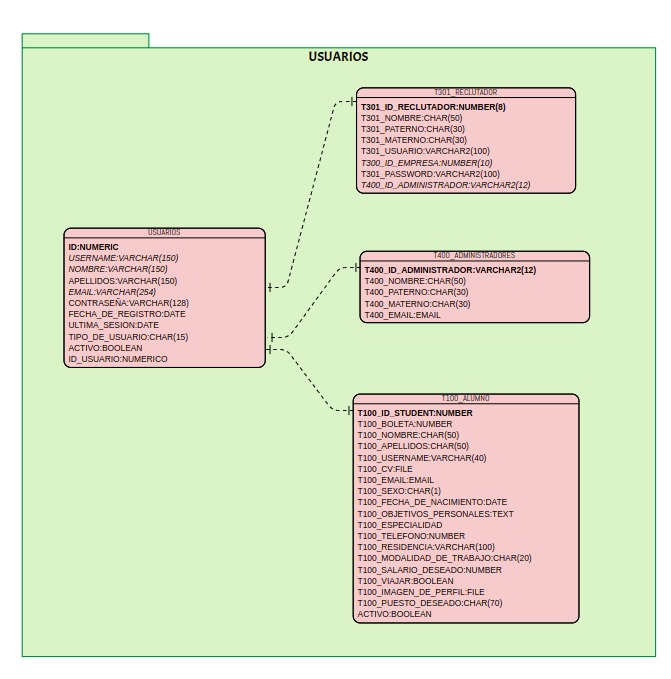
\includegraphics[width=.6\textwidth]{anexos/imagenes/Usuarios.jpeg}
            
    \end{center}
        \label{fig:MI-Planeacion}
            \caption{Diagrama de base de datos del módulo de Usuarios}
    
    \end{figure}

% En la figura  \ref{fig:MI-PlaneacionI}
%\begin{figure}[hbtp!]
%    \begin{center}
%        \includegraphics[width=.7\textwidth]{negocio/images/MI-POA-CAT}
%    \end{center}
%    \label{fig:MI-PlaneacionI}
%\end{figure}
%
%\begin{figure}[hbtp!]
%    \begin{center}
%        \includegraphics[width=.7\textwidth]{negocio/images/MI-POA-CFG}
%    \end{center}
%    \label{fig:MI-PlaneacionII}
%\end{figure}
%
%\begin{figure}[hbtp!]
%    \begin{center}
%        \includegraphics[width=.7\textwidth]{negocio/images/MI-POA-PLA}
%    \end{center}
%    \label{fig:MI-PlaneacionIII}
%\end{figure}



%---------------------Ejercicio Fiscal---------------------

\begin{cdtEntidad}{users}{Usuario}{
    Es un periodo de tiempo, generalmente de 12 meses donde las Alcaldías, Dependencias, Órganos Desconcentrados y Entidades, cuadran las cuentas de sus actividades financieras y contables.}

	    \brAttr{id}{Id}{tInt}{
	        Es el correo del alumno con el cual se identificara como unico dentro del sistema.
	        Restricciones adicionales:
            \begin{Citemize}
                \item \refElem{tPrimaryKey}
                \item \refElem{tUnico}
            \end{Citemize}
        }{\datRequerido}

        \brAttr{password}{Contraseña}{tVarchar}{
	        Es el correo del alumno con el cual se identificara como unico dentro del sistema.
        }{\datRequerido}

        \brAttr{username}{User Name}{tVarchar}{
	        Es el correo del alumno con el cual se identificara como unico dentro del sistema.
	        Restricciones adicionales:
            \begin{Citemize}
                \item \refElem{tUnico}
            \end{Citemize}
        }{\datRequerido}

       % \brAttr{t100_email}{Nombre }{tEmail}{
	   %     Es el correo del alumno con el cual se identificara como unico dentro del sistema.
	   %     Restricciones adicionales:
       %     \begin{Citemize}
       %         \item \refElem{tPrimaryKey}
       %         \item \refElem{tUnico}
       %     \end{Citemize}
       % }{\datRequerido}

      %  \brAttr{t100_email}{Apellidos}{tEmail}{
	   %     Es el correo del alumno con el cual se identificara como unico dentro del sistema.
	   %     Restricciones adicionales:
       %     \begin{Citemize}
       %         \item \refElem{tPrimaryKey}
       %         \item \refElem{tUnico}
       %     \end{Citemize}
       % }{\datRequerido}

       % \brAttr{t100_email}{Fecha de registro}{tEmail}{
	   %     Es el correo del alumno con el cual se identificara como unico dentro del sistema.
	   %     Restricciones adicionales:
       %     \begin{Citemize}
       %         \item \refElem{tPrimaryKey}
       %         \item \refElem{tUnico}
       %     \end{Citemize}
       % }{\datRequerido}

       % \brAttr{t100_email}{Last login}{tdate}{
	   %     Es el correo del alumno con el cual se identificara como unico dentro del sistema.
	   %     Restricciones adicionales:
       %     \begin{Citemize}
       %         \item \refElem{tPrimaryKey}
      %          \item \refElem{tUnico}
       %     \end{Citemize}
       % }{\datRequerido}

       % \brAttr{t100_email}{Super usuario}{bolean}{
	   %     Es el correo del alumno con el cual se identificara como unico dentro del sistema.
	   %     Restricciones adicionales:
       %     \begin{Citemize}
       %         \item \refElem{tPrimaryKey}
       %         \item \refElem{tUnico}
       %     \end{Citemize}
       % }{\datRequerido}

       % \brAttr{t100_email}{Stado}{bolean}{
	   %     Es el correo del alumno con el cual se identificara como unico dentro del sistema.
	   %     Restricciones adicionales:
       %     \begin{Citemize}
       %         \item \refElem{tPrimaryKey}
       %         \item \refElem{tUnico}
       %     \end{Citemize}
       % }{\datRequerido}

       % \brAttr{t100_email}{user_id}{bolean}{
	   %    
       %     \begin{Citemize}
       %         \item \refElem{tPrimaryKey}
       %         \item \refElem{tUnico}
       %     \end{Citemize}
       % }{\datRequerido}
        
       % \brAttr{t100_email}{user_type}{bolean}{
	    %   
        %    \begin{Citemize}
       %         \item \refElem{tPrimaryKey}
       %         \item \refElem{tUnico}
       %     \end{Citemize}
       % }{\datRequerido}

	   
\end{cdtEntidad}
